\section{Model inference}
\label{sec:related:modelinf}

In the Industry, software models as defined in
\crossref{sec:related:testing}{sec:related:testing:model} are
often neglected: specifications are not up to date (or even
missing), models are neither accurate nor sound, and also rarely
formals.

Such a situation can be comprehensible because writing complete
documentation and especially formal models is often a tedious and
error prone task. That is why lightweight models are usually
found in the Industry. This leads to several issues, e.g., the
toughness of validating applications with a good test coverage,
or the difficulty to diagnose failures or to maintain them since
they are poorly documented.

A solution to these problems is to infer models. Model
inference is a research field that aims at (automatically)
creating models, expressing functional behaviors of existing
applications.  These models, even if incomplete (or partial),
help understand how an application behaves. They can be generated
from execution traces (sequences of observed actions)
\cite{Krka:2010:UDE:1810295.1810324}, documentation
\cite{ZhongZXM11}, source code
\cite{Salah05scenariographer,Pradel:2009}, and even network
traces \cite{6079839} or more abstract languages such as WSDL
description \cite{Bertolino:2009:ASB:1595696.1595719}. Although
this area sounds promising, it exposes several open problems that
require further investigation. Among them, the most known problem
is that the model generation may lead to a state space explosion
problem. Some works construct lightweight models to avoid this
issue \cite{WPX13}, others yield extrapolated models by merging
application's states that, unfortunately, express more or
slightly different behaviors than those observed \cite{4023976}.

Model inference is employed for different purposes. One can infer
model from log files in order to retrieve important information
to identify failure causes \cite{4700316}. It has also
successfully been applied to intrusion detection \cite{debar00},
searching for features in execution traces that allow to
distinguish browsers from other software systems, using
automatically generated finite automata.
A prominent use of model inference is Model-Based Testing (MBT)
and verification, leading to numerous techniques to automate
testing, e.g., with crawlers
\cite{Amalfitano:2012:UGR:2351676.2351717,Joorabchi:2012:REI:2420240.2420457,MobiGUITARIEEESoftware2014}.
One of the key elements of MBT is the model that describes the
behavior of the system under test (SUT). Such a model is supposed
to provide an abstract view of the SUT by focusing on specific
aspects, e.g., the change of a system state at runtime.

In the literature, we can find different techniques to infer
models that can be organized in two main categories. Some
techniques infer models by assuming a set of traces available for
learning the models. We refer to this principle as passive
learning since they don't directly interact with the system to
learn a model. In the second category, we find the techniques
that don't assume a fixed set of traces available at the
beginning of the model inference process. Indeed, learning
algorithms but also crawlers enable the possibility to actively
learn models by interacting with the system to model.

In the following Section, we give an overview of prominent active
learning techniques: introducing $\EuScript{L}^*$-based
techniques, incremental learning techniques, and crawling
techniques.
Passive learning techniques are extensively described in Section
\ref{sec:passive}, covering Finite State Automaton (FSA)
inference techniques, state invariant methods, white-box
approaches, and we add a few alternative techniques.

%%%%%%%%%%%%%%%%%%%%%%%%%%%%%%%%%%%%%%%%%%%%%%%%%%%%%%%%%%%%%%%%%

\subsection{Active learning}
\label{sec:active}

\begin{figure}[h]
    \begin{center}
        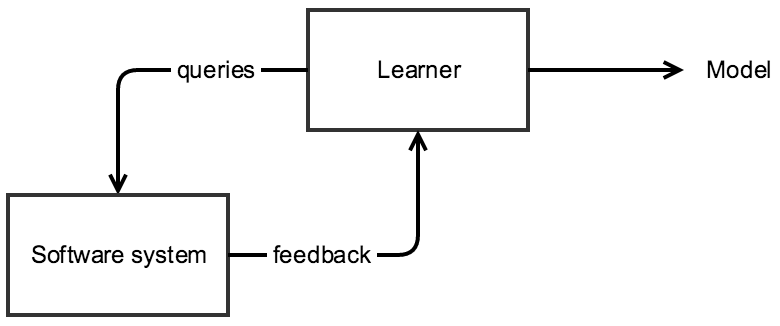
\includegraphics[width=0.9\linewidth]{figures/active.png}
    \end{center}

    \caption{Active learning big picture.}
    \label{fig:active}
\end{figure}

Active learning algorithms actively interact with the system to
learn models \cite{settles.tr09}. Instead of relying on given
traces, these algorithms (a.k.a. \textit{Learners}) ask questions
(a.k.a.  queries) to an \textit{Oracle} and a \textit{Teacher},
e.g., users or test engines. A learner can then use this feedback
to improve a model as depicted in Figure \ref{fig:active}.
Moreover, by asking informative queries (e.g., close to the
decision boundary), an active learner potentially requires much
less examples than a passive learner that learns from data
samples as we will see in Section \ref{sec:passive}. Here, we
focus on methods that ask queries to software systems, which we
decided to extend by incorporating some crawling techniques
originating from the automated Graphical User Interface (GUI)
testing field.

Most of the existing active learning techniques have been
initially conceived upon two concepts: the $\EuScript{L}^*$
algorithm, presented in Section \ref{sec:active-letoile}, and
incremental learning, presented in Section
\ref{sec:active-increment}. However, as said above, some works
use crawling techniques to infer models and can be categorised as
active learning techniques too. We introduce some of them in
Section \ref{sec:active-crawling}.

\subsubsection{$\EuScript{L}^*$-based techniques and related}
\label{sec:active-letoile}

\begin{figure}[h]
    \begin{center}
        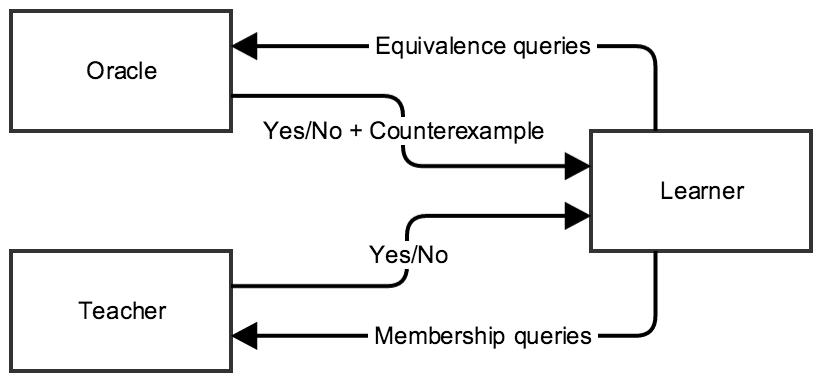
\includegraphics[width=0.9\linewidth]{figures/angluin.png}
    \end{center}

    \caption{The principle of $\EuScript{L}^*$-based learning
    algorithms.}
    \label{fig:angluin}
\end{figure}

The $\EuScript{L}^*$ algorithm by Angluin \cite{Angluin198787} is
a well-known active learning method that can learn models of
black box implementations. We assume here that a system can be
modeled by a Deterministic Finite Automata (DFA) $\EuScript{A}$,
and we are interested in constructing a model
$\EuScript{L}(\EuScript{A})$ that is equivalent to $\EuScript{A}$
(in the literature, this is known as identifying the regular
language which is accepted by $\EuScript{A}$). A learner, who
knows nothing about $\EuScript{A}$, is trying to learn
$\EuScript{L}(\EuScript{A})$ by asking queries to a teacher and
an oracle by means of two kinds of queries, as depicted in Figure
\ref{fig:angluin}:

\begin{itemize}
\item a \textit{membership query}, consisting in asking the
teacher whether a word is contained in the regular language;

\item an \textit{equivalence query}, consisting in asking the
oracle whether a hypothesized DFA $\EuScript{M}$ is correct, i.e.
$\EuScript{L}(\EuScript{M}) = \EuScript{L}(\EuScript{A})$.  The
oracle either answers $yes$ or $no$ along with a counterexample.
\end{itemize}

By taking the counterexample into account, the $\EuScript{L}^*$
algorithm iterates by asking new queries and constructing a new
hypothesized DFA $\EuScript{M}$, until it gets an automaton that
is equivalent to the black box.  This method is interesting but
requires a lot of iterations and heavy use of an expert oracle.
It is designed for complete rather than incremental learning.

The work described in \cite{Alur:2005:SIS:1047659.1040314}
generates behavioral interface specifications for Java classes by
means of predicate abstraction and active learning. This is a
white-box approach inspired by
\cite{Whaley:2002:AEO:566171.566212} (see Section
\ref{sec:passive-white}) that, first, uses \textit{predicate
abstraction} to generate an abstract version of the considered
class. Afterwards, a minimal version (interface) of this
abstraction is constructed by leveraging the $\EuScript{L}^*$
algorithm. The tool \textit{Java Interface Synthesis Tool} (JIST)
is the resulting implementation of such a technique. It takes
Java classes as input, and generates useful and safe interfaces
automatically.

Raffelt et al. introduced \textit{LearnLib}
\cite{Raffelt:2005:LLA:1081180.1081189}, a library for learning
deterministic finite state automata. It implements the
$\EuScript{L}^*$ \cite{Angluin198787} learning algorithm for
inferring DFA and some slight variants for deriving Mealy
machines \cite{6771467}, which has been formally proposed by
Niese in \cite{DBLP:phd/de/Niese2003}.  Raffelt et al. added a
feature called \textit{filters} to the classical learning
algorithm in order to exploit domain specific properties to
actively reduce the number of queries that a teacher is asked
during a learning phase.
Additionally, statistical data acquisition can be employed to
evaluate the learning procedure. These features make
\textit{LearnLib} a powerful tool if a teacher is available and
DFA are the target model of choice.  Merten et al. revisited
\textit{LearnLib} in a tool called \textit{Next Generation
LearnLib} (NGLL) \cite{ngll11}, a machine learning framework
providing infrastructure for practical application, including the
tool \textit{LearnLib Studio}, a graphical interface for
designing and executing learning and experimentation setups, plus
a set of Java libraries. Howar et al. inferred \textit{semantic
interfaces} of data structures on the basis of systematic testing
in \cite{howar2012}. Semantic interfaces transparently reflect
the behavioral influence of parameters at the interface level.
They defined \textit{Register Mealy Machines} (RMMs) to express
the data structures behavior concisely, but also because RMMs can
be learnt much more efficiently than both \textit{Register
Automata} and plain Mealy machines at a given level of
abstraction. Register automata, also known as \textit{Finite
Memory Automata} \cite{Kaminski1994329}, are models that are
capable of expressing the influence of data on control flow.
Howar et al. proposed a technique and an implementation on top of
\textit{LearnLib} to actively learn register automata in
\cite{howarRA2012}. For further information, active learning of
Mealy machines has extensively been covered in \cite{steffen11}.

Walkinshaw et al. presented the \textit{Query-driven State
Merging} (QSM) algorithm in
\cite{Walkinshaw07reverseengineering}, an \textit{interactive}
grammar inference technique to infer the underlying state machine
representation of an existing software system. The approach is
said interactive because it generates queries to the user as it
constructs a hypothesis machine that can be interpreted as
tests. It is similar to the work done by Hungar in \cite{hungar},
who used the $\EuScript{L}^*$ algorithm, but the QSM
algorithm presumes that the input sequences offer some basic
coverage of the essential functionality of the system, in which
case the machine can be inferred relatively cheaply by a process
of state merging, compared to the $\EuScript{L}^*$ technique that
systematically and comprehensively explore the state space of the
target machine. It is worth mentioning that QSM does not aim at
learning the complete automaton but, rather, to generalize the
supplied traces. It can be supplied a subset of traces with
interesting behaviors, and it will generalize from these using
queries. Some tools such as \textit{Synapse}
\cite{LamelaSeijas:2014:SAB:2633448.2633457} implement the QSM
algorithm to perform automatic behavior inference and
implementation comparison for the programming language Erlang.

Berg et al. also revisited the $\EuScript{L}^*$ algorithm in
\cite{regularinfBerg06}, by generalizing it so that it can infer
a partially defined automaton, and by defining a mechanism for
inferring guards of a parameterized system from the symbols in an
underlying partially defined automaton (by replacing the
representative symbols by guards that characterize the
transitions represented by each symbol). This new algorithm is
intended to infer parameterized systems where guards of
transitions use only a small subset of all parameters of a
particular action type. Such a work has been used later to infer
state machines for systems with parameterized inputs
\cite{regularinfBerg08}. Here, authors inferred a behavioral
model (finite-state Mealy machine) for a finite data domain, and
then, abstracted this model to a symbolic Mealy machine, encoding
extrapolated invariants on data parameters as guarded
transitions.

A common problem to the algorithms presented above is the time
spent querying the oracle or the teacher, that is why many works
proposed \textit{incremental} versions of them.

\subsubsection{Incremental learning algorithms}
\label{sec:active-increment}

Incremental learning algorithms play an important role in
situations where all the training examples are not available to
the learner at the start. A learning algorithm is incremental if:
(i) it constructs a sequence of hypothesis automata $H_0, \dots,
H_n$ from a sequence of observations $o_0, \dots, o_n$  about an
unknown automaton $A$, and (ii) the construction of hypothesis
$H_i$ can reuse aspects of the construction of the previous
hypothesis $H_{i-1}$.

Dupont proposed an incremental extension of the Regular Positive
and Negative Inference (RPNI) algorithm known as the
\textit{Regular Positive and Negative Incremental Inference}
(RPNI2 or RPNII) algorithm in \cite{Dupont96incrementalregular}.
Initially, the inference process of the RPNI algorithm had to be
restarted from scratch when new learning data were available. The
RPNII algorithm overcomes this limitation by dealing with
sequential presentation, i.e. the learning data are presented one
at a time in a random order.

Similarly, Parekh et al. \cite{parekh98} proposed an incremental
extension of Angluin's \textit{ID} algorithm \cite{ANGLUIN198176}
(which is not incremental since only a single hypothesis
automaton is ever produced) for learning DFA from labeled
examples and membership queries known as \textit{Incremental ID}
(IID). IID is guaranteed to converge to the target DFA and has
polynomial time and space complexities. Sindhu et al. also
enhanced the ID algorithm by proposing another incremental
version of it, called \textit{Incremental Distinguishing
Sequences} (IDS) \cite{journals/corr/abs-1206-2691}, that uses
the distinguishing sequence technique for incremental learning of
DFA. In contrast with IID, the IDS algorithm, and its proof of
correctness are much simpler.

Meinke introduced an algorithm for sequential learning of Mealy
automata by \textit{Congruence Generator Extension} (CGE) in
\cite{meinkeCGE}. The term \textit{sequential} indicates that
this algorithm can produce a sequence of hypothesis automata
$\EuScript{A}_0, ..., \EuScript{A}_n$ which are approximations to
an unknown automaton $\EuScript{A}$, based on sequence of
information (queries and results) about $\EuScript{A}$. A
sequential algorithm is said \textit{incremental} if computation
of successive approximations can reuse previous results (more
information can be found in \cite{Parekh00grammarinference}) as
stated previously.  Using finitely generated congruences here
increases the efficiency of hypothesis automaton representation.
The CGE algorithm has some features in common with the RPNII
algorithm mentioned previously: both RPNII and CGE perform a
recursive depth first search of a lexicographically ordered state
set with backtracking. However, RPNII is designed for Moore
machines with binary outputs (positive/negative), while CGE is
coded for Mealy machines.

Some incremental learning algorithms, such as those which are
both sequential and incremental, can be specifically chosen to
make testing more effective and scalable. That is the case of
several works on \textit{Learning-Based Testing} (LBT). For
example, Meinke and Sindhu \cite{tap2011} introduced an
incremental learning algorithm named \textit{Incremental Kripke
Learning} (IKL) for Kripke structures modeling reactive systems.

In the next Section, we present some other works that infer
models by interacting with software systems by exploring them.

\subsubsection{Crawling techniques through Graphical User Interfaces}
\label{sec:active-crawling}

\begin{figure}[ht]
    \begin{center}
        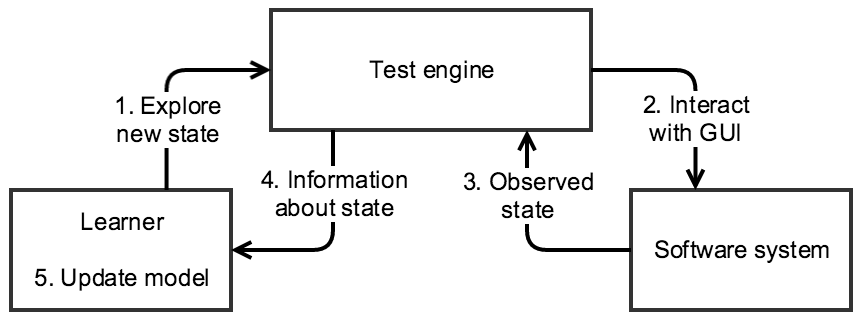
\includegraphics[width=0.9\linewidth]{figures/crawler.png}
    \end{center}

    \caption{The principle of inferring models with crawling
    techniques.}
    \label{fig:crawler}
\end{figure}

A lot of different works, which originate from automatic
black-box testing, retrieve specifications of event-driven
applications (either desktop, web, or mobile) by exploring them
(in other words, crawling them). Learning is achieved by
stimulating the application and gathering all the events in a
model as depicted in Figure \ref{fig:crawler}. While the
techniques presented in the two previous Sections try to learn an
exact model reflecting counterexamples, the works presented below
don't always learn from counterexamples. However, they all crawl
the applications in order to infer models.

Memon et al. initially presented \textit{GUITAR} in
\cite{Memon:2003}, a tool for scanning desktop applications that
produces event flow graphs and trees showing the Graphical User
Interface (GUI) execution behaviors. The generated models are
quite simple and many false event sequences have to be weeded out
later.

Mesbah et al. proposed the tool \textit{Crawljax}
\cite{crawljax:tweb12}, specialised in AJAX applications, i.e.
dynamic web applications.  It produces a state machine model to
capture the changes of the DOM structures of HTML documents
obtained after triggering events (click, mouseover, etc.). An
interesting feature of Crawljax is the concatenation of identical
states in the model under construction, by comparison based on
the DOM structure. In practice, the model encompasses all the
actions performed by the implementation. To avoid a state
explosion problem, state abstractions should be manually given.
\textit{WebMate} \cite{webmate12} is another, more recent, model
extractor for web applications. This tools learns a \textit{usage
model} that captures how a user can interact with the web
application, modeling all the interactions as a graph where
nodes correspond to different states of the application, and
edges represent user interactions.

More recently, crawlers for mobile applications were proposed in
\cite{Amalfitano:2012:UGR:2351676.2351717,Joorabchi:2012:REI:2420240.2420457,MobiGUITARIEEESoftware2014}.
These provide simple trees, depicting the observed GUI. In
\cite{Amalfitano:2012:UGR:2351676.2351717}, Amalfitano et al. use
ripping to automatically and systematically traverse the
application's user interface, generating and executing test cases
as new events are encountered. Their technique relies on a state
machine model of the GUI, called a GUI tree, containing the set
of GUI states and state transitions encountered during the
ripping process.  Later, Amalfitano et al. also created
\textit{MobiGUITAR} \cite{MobiGUITARIEEESoftware2014}, an
adaptation of the GUITAR tool for automated GUI-driven testing of
Android applications. Here, the abstraction is a scalable
state-machine model that represents the application's GUI as in
\cite{Amalfitano:2012:UGR:2351676.2351717}. In a similar manner,
Joorabchi et al. presented a reverse engineering technique that
creates state flow graphs of iOS applications in
\cite{Joorabchi:2012:REI:2420240.2420457}.

Yang et al. \cite{WPX13} presented a grey-box testing method for
Android applications whose originality lies in the static
analysis of the code to only infer the events that can be applied
to the GUI later. Then, a classical crawling technique is
employed to derive a lightweight models (simple trees). The
exploration can be directed either in breadth-first order or in
depth-first order.

More recently Choi et al. introduced an algorithm to generate
finite state machines \cite{Choi2013}, in conjunction with a
testing approach.  Their testing engine aims at interacting with
the application under test to discover new application states,
and to build a model accordingly. If an input sequence
contradicts the learnt model, the learning algorithm rebuilds a
new model that meets all the previous scenarios. They proposed a
novel Learning-Based Testing algorithm that avoids restarts and
aggressively merges states in order to quickly prune the state
space, so that it outperforms $\EuScript{L}^*$-based testing.

In the following Section, we present our second category of model
inference techniques, which don't interact with the software
system to learn models but rather, infer models from execution
traces.

%%%%%%%%%%%%%%%%%%%%%%%%%%%%%%%%%%%%%%%%%%%%%%%%%%%%%%%%%%%%%%%%%

\subsection{Passive learning}
\label{sec:passive}

\begin{figure}[h]
    \begin{center}
        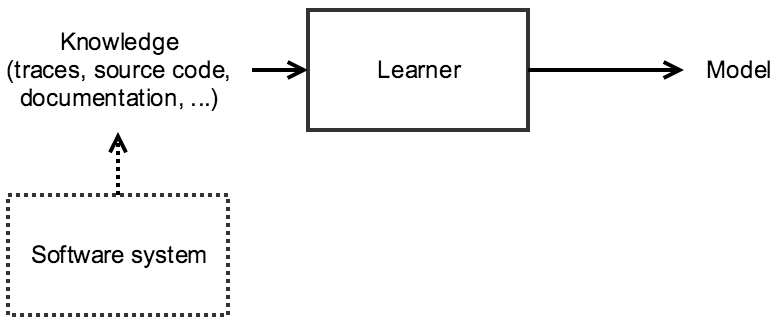
\includegraphics[width=0.9\linewidth]{figures/passive.png}
    \end{center}

    \caption{Passive learning big picture.}
    \label{fig:passive}
\end{figure}

For passive learning techniques, a model is inferred from a fixed
set of knowledge, such as a set of execution traces, source code,
and even documentation. The algorithms are designed to construct
models based on this fixed set of positive (and possibly
negative) examples only as shown in Figure \ref{fig:passive}.

We cover Finite State Automaton inference in Section
\ref{sec:passive-fsa} since these works are prominent in passive
learning model inference. Such techniques use behavioral
equivalence to merge states in order to construct models.
We then present techniques that use invariants to merge states in
Section \ref{sec:passive-spec}. Some white-box techniques used to
infer models are presented in Section \ref{sec:passive-white},
and a few alternative works are introduced in Section
\ref{sec:passive-others}.

\subsubsection{FSA inference techniques}
\label{sec:passive-fsa}

The approaches to infer Finite State Automata (FSA) aim at
comprehensively describing method execution sequences from a set
of dynamic method invocation traces.

Most existing approaches for FSA inference are based on the
\textit{kTail} algorithm \cite{5009015}. This algorithm generates
a FSA from a set of traces in two steps.  First, it builds a
Prefix Tree Acceptor (PTA), which is a tree where edges are
labeled with event names.  The language accepted by the PTA
exactly consists of the set of event sequences recorded in the
traces. Then, kTail transforms the PTA into a FSA by merging two
states if they share the same future of length $k$. The future of
length $k$ of a state is defined as the set of the event
sequences of maximum length $k$ that can be accepted from the
state. The final automaton is obtained by merging every pair of
states with the same future of length $k$.

However, kTail for complex software systems can produce imprecise
and overgeneralized models containing undesirable behaviors
\cite{4023976}. Reiss and Renieris improved the kTail algorithm
by proposing a new algorithm which merges two states if they
share at least one \textit{k-future} \cite{919096}. By using a
merging criterion that is weaker than the kTail, their variant
merges more states than kTail.
Lo et al. \cite{Lo:2009:ASB:1595696.1595761} also enhanced the
kTail algorithm by incorporating state information. They
proposed to, first, inferring temporal properties that generally
hold for the dynamic traces, and then, merging states, while
ensuring that the merge does not violate the inferred properties.
However, this approach only considers the observed execution
sequences and does not consider internal state information.
Lorenzoli et al. also extended kTail to produce FSAs with
transitions annotated by algebraic constraints
\cite{Lorenzoli2008}. Their technique, called \textit{gkTail},
generates an EFSA from a set of traces that incorporate
information about both the event sequences and the values of the
parameters associated with event sequences.

Another algorithm for inferring FSAs is the \textit{kBehavior}
\cite{mariani2007dynamic}. It incrementally generates a FSA from
a set of traces. When a new trace is submitted to kBehavior, this
algorithm first identifies sub-traces of the input trace that are
accepted by sub-automata in the current automaton (the sub-traces
must have a minimal length \textit{k}, otherwise they are
considered too short to be relevant). Then, kBehavior extends the
automaton with the addition of new branches that suitably connect
the identified sub-automata, producing a new version of the
automaton that accepts the entire input trace. They successfully
applied this algorithm to automatically analyse log files and
retrieved important information to identify failure causes
\cite{4700316}. They also automatically analysed logs obtained
from workloads to highlight useful information that can relate
the failure to its cause \cite{cotroneo2007investigation}.  Both
works describe the \textit{kLFA} technique that generates an FSA
from a set of traces that incorporate information about both the
event sequences and the values of the attributes associated with
events. The generated FSA has special transition labels that
include data flow symbols.

Lo et al. evaluated kTail, kBehavior, gkTail, and kLFA with a set
of 10 case studies extracted from real software systems in
\cite{Lo20122063}. This empirical comparative study quantifies
both the effect of adding data flow information within automata
and the effectiveness of the techniques when varying sparseness
of traces. One of the main conclusions is that adding algebraic
constraints to FSAs does not compromise quality but negatively
affects performance. This is the case of gkTail for instance,
which is extremly slow. The study also revealed that having more
traces is important but not enough because these algorithms have
difficulties to control over-generalization.

The techniques presented in this Section are focused on building
specifications modeled as Finite State Automata. However, the
execution traces often provide a highly detailed but limited
subset of the possibly infinite set of legal executions. This is
a barrier for inferring exact models.
That is why other techniques, such as state invariant methods for
instance, have been employed to overcome this limitation. In the
next Section, we present some of these state invariant
techniques.


\subsubsection{State invariant techniques}
\label{sec:passive-spec}

Ammons et al. first introduced the term \textit{specification
mining} \cite{Ammons:2002:MS:565816.503275} to describe a machine
learning technique that infers a specification by observing
software system execution and concisely summarizing the frequent
interaction patterns as state machines that capture both temporal
and data dependences. These state machines can be examined by a
developer, to refine the specification and identify errors, and
can be utilized by automatic verification tools to find bugs.

Ernst et al. proposed automatic deduction of formal
specifications from execution traces
\cite{Ernst:1999:DDL:302405.302467}. Their \textit{Daikon} tool
works by learning likely invariants involving software variables
from dynamic traces. An invariant is a property that holds at a
certain point or points in a software. These are often used in
assert statements, documentation, and formal specifications.
Dynamic invariant detection runs a software system, observes the
values that the software computes, and then reports properties
that were \textit{true} over the observed executions.  This is a
machine learning technique that can be applied to arbitrary data.
Daikon's output has been used for generating test cases,
predicting incompatibilities in component integration, automating
theorem proving, repairing inconsistent data structures, and
checking the validity of data streams, among other tasks
\cite{Ernst200735}.  In \cite{Krka:2010:UDE:1810295.1810324},
Krka et al. inferred object level behavioral models from
dynamically observed executions, by using not only execution
traces but also dynamically inferred invariants. That way, they
proposed a better technique to infer FSA than those presented in
Section \ref{sec:passive-fsa}.

Yang et al. \cite{Yang:2006:PMT:1134285.1134325} created
\textit{Perracotta}, an inference engine for temporal API rules
that is able to scale to large software systems and work
effectively with the imperfect traces typically available in
industrial scenarios, using an approximate inference algorithm.
They developed an analysis technique for detecting dominant
behaviors from a software system's potentially imperfect traces,
and introduced heuristics for automatically identifying
properties that are likely to be interesting.

In \cite{Ghezzi:2009:SIB:1555001.1555057}, Ghezzi et al.
described an approach (\textit{SPY}) to recover the specification
of a software component from the observation of its runtime
behavior. They infer a formal specification of stateful black-box
components that behave as data abstractions by first, building a
Deterministic Finite Automaton (DFA) that models the partial
behavior of instances of the data abstraction, and then, by
generalizing it via graph transformation rules. The rules can
generate a possibly infinite number of behavioral models though.

Taking another direction by leveraging genetic algorithms,
Tonella et al. \cite{TonellaNMLH13} applied a data-clustering
algorithm to execution traces with concrete states in order to
group concrete states into clusters. They then run invariant
inference on each cluster to infer a set of invariants for each
cluster as in \cite{Ernst:1999:DDL:302405.302467,Ernst200735},
and they iteratively improve the clustering, using a genetic
algorithm, so as to optimize the quality attributes of the
associated Finite State Machine (FSM) model. Each distinct set of
invariants produced for each cluster at the end of the
optimization represents an abstract state and is used as the
abstraction function that maps concrete states to abstract ones.
By applying these abstraction functions to concrete input traces
they are able to generate the output model.

The works presented in this Section are either grey- or black-box
techniques. Next Section introduces some passive inference
techniques that use a white-box approach.


\subsubsection{White-box techniques}
\label{sec:passive-white}

Here, we are interested in techniques that infer models from
source code. While the source code is available to the learner or
the source code is instrumented at runtime, the learner does not
interact with the system by querying it.

Whaley et al. proposed using multiple FSM submodels to model the
interface of a class in \cite{Whaley:2002:AEO:566171.566212}. Two
techniques are given to automatically construct such models: a
dynamic instrumentation technique, and a static analysis that
infers pairs of methods that cannot be called consecutively,
leading to a DFA with one state per method. A more general and
formal solution to interface synthesis is given in
\cite{Alur:2005:SIS:1047659.1040314} (and covered in Section
\ref{sec:active-letoile}).

Salah et al. proposed \textit{Scenariographer}
\cite{Salah05scenariographer}, an algorithm and a tool to
estimate the usage scenarios of a class from its execution
profile. The estimation process produces canonical groups, where
each group comprises a set of similar method invocation sequences
that represent a usage scenario.

Later, Shoham et al. introduced an approach to mine temporal API
specifications based on static analysis in
\cite{Shoham:2007:SSM:1273463.1273487}. They proposed a two-step
approach: (i) an abstract-trace collection to collect sets of
possible behaviors in client software, and (ii) a summarization
phase to filter out noise. Mined specifications are often too
detailed here, and their solution does not scale well. The
scaling problem is fundamental to all software analyses and is
discussed in Section \ref{sec:discussion:limitations}.

In \cite{Pradel:2009}, Pradel and Gross presented a scalable
dynamic analysis that infers extremely detailed specifications of
correct method call sequences on multiple related objects. Their
approach preprocesses method traces to identify small sets of
related objects (object collaborations) and method calls which
can be analysed separately. Then, they derive temporal
specifications. This work has been extended in
\cite{Dallmeier_generatingtest} by means of active testing.

In \cite{Wasylkowski07detectingobject}, Wasylkowski et al.
proposed \textit{JADET}, a Java code analyser to infer sequences
of method calls. These sequences are then used to produce object
usage patterns that serve to detect object usage violations in
the code. This is similar to
\cite{Wasylkowski_miningoperational}, which introduced
\textit{OP-Miner}, a tool that learns and checks operational
preconditions of methods by static software analysis.

The methods described in \cite{concolicandroid12,5416728} rely
upon concolic testing to explore symbolic execution paths of the
application and to detect bugs. In \cite{concolicandroid12},
Anand et al. presented an algorithm for generating input events
to exercise smartphone applications, symbolically tracking events
from the point where they originate to the point where they are
ultimately handled. In \cite{5416728}, Artzi et al. proposed a
technique to generate tests for web applications, relying on both
combined concrete and symbolic execution and explicit state model
checking. These white-box approaches theoretically offer a better
code coverage than black-box automatic testing. However, the
number of paths being explored concretely limits to short paths
only, and the constraints have not to be too complex for being
solved.


\subsubsection{Alternative techniques}
\label{sec:passive-others}

Some other passive learning techniques rely on another set of
knowledge to infer models, such as documentation for instance,
and a few others leverage different techniques altogether to
construct models. In this Section, we present some of these
works.

Bertolino et al. presented \textit{StrawBerry} in
\cite{Bertolino:2009:ASB:1595696.1595719}, a method that infers a
\textit{Behavior Protocol} automaton from a Web Service
Description Language (WSDL) document.  WSDL is a format for
documenting a variety of Web Services, containing information
about the inputs, outputs and available operations. StrawBerry
automatically derives a partial ordering relation among the
invocations of the different WSDL operations, that is represented
as an automaton called Behavior Protocol automaton.  This
automaton models the interaction protocol that a client has to
follow in order to correctly interact with the Web Service.  The
states of the behavior protocol automaton are Web Service
execution states and the transitions, labeled with operation
names and input/ouput data, model possible operation invocations
from the client of the Web Service.

Later, Zong et al. \cite{ZhongZXM11} proposed to infer
specifications from API documentation to check whether
implementations match it.  Such specifications do not reflect the
implementation behavior though. Furthermore, this method can be
applied only if these API documentations are available in a
readable format.
